% Copyright 2026 Sreeram Anil
% SPDX-License-Identifier: CC-BY-4.0
% =============================================================================
%  Steady-state Kalman filter / LQE observer
% =============================================================================
\chapter{Steady-State Kalman (LQE) Observer (SSKF)}
\label{ch:sskf}

\section*{At a glance}
\begin{tabular}{@{}l>{\raggedright\arraybackslash}p{0.76\textwidth}@{}}
Family & Deterministic observers \\
Header & \texttt{include/estkit/observers/luenberger.hpp} (\texttt{design = Riccati}) \\
Registered name & \texttt{SSKF} \\
State dimension & $n_x = 4$ (cell model) --- generic in $n_x, n_u, n_y$ \\
Cost per step & $\mathcal{O}(n_x^2)$ steady state; one DARE solve at reset; $\approx 0.5\,\mu$s/step measured \\
Primary references & \cite{kalman1960,andersonmoore1979,luenberger1971,simon2006} \\
\end{tabular}

\section{Motivation and aerospace/BMS relevance}
The Kalman filter's gain sequence $\mK_k$ converges, for a time-invariant detectable and
stabilisable pair, to a constant $\mK_\infty$ \cite[Sec.~4.4]{andersonmoore1979}.  Once it has
converged, propagating $\mP_k$ every sample buys nothing except the covariance output.  The
steady-state Kalman filter --- in the control literature, the \emph{linear quadratic estimator} --
throws the recursion away and keeps $\mK_\infty$.

This is the standard industrial compromise and it is everywhere in flight hardware: the
complementary filters in inertial systems, the fixed-gain attitude estimators of small UAVs, and
most shipping BMS SOC estimators are steady-state Kalman filters in disguise.  The reasons are
the same as for the Luenberger observer (\Cref{ch:luenberger}) --- bounded execution time, no
covariance to corrupt --- with one addition: the gain is not an arbitrary design choice but the
one that minimises the stationary error variance under the model's own $\mQ$ and $\mR$.  When a
BMS supplier can defend $\mQ$ and $\mR$ from sensor datasheets, that is a much easier
certification story than ``we chose $\tau = 60$\,s''.

The SSKF is registered from the same class as the Luenberger observer with
\texttt{design = Riccati}; the two registrations therefore isolate exactly one variable, the
origin of the gain, and the benchmark comparison between them is a controlled experiment.

\section{Problem statement and assumptions}
The plant is \eqref{eq:lue-plant-f}--\eqref{eq:lue-plant-h} with the additional assumption that
$\vw_k$ and $\vv_k$ are zero-mean, mutually uncorrelated white sequences with
\begin{equation}
\E{\vw_k\vw_k^\T} = \mQ(\vx,\vu), \qquad \E{\vv_k\vv_k^\T} = \mR(\vx,\vu) ,
\label{eq:sskf-noise}
\end{equation}
both supplied by the model.  We additionally require $(\mA,\mC)$ detectable and
$(\mA,\mQ^{1/2})$ stabilisable, which guarantee a unique stabilising solution of the discrete
algebraic Riccati equation.

\section{Derivation}

\subsection{The algebraic Riccati equation}
Let $\Pminus_k = \E{(\xminus_k-\vx_k)(\xminus_k-\vx_k)^\T}$.  The Kalman recursion in
current-estimator form is
\begin{align}
\mS_k &= \mC\Pminus_k\mC^\T + \mR , \label{eq:sskf-S}\\
\mK_k &= \Pminus_k\mC^\T\mS_k\inv , \label{eq:sskf-K}\\
\Pminus_{k+1} &= \mA\big(\Pminus_k - \mK_k\mC\Pminus_k\big)\mA^\T + \mQ . \label{eq:sskf-riccati}
\end{align}
For a time-invariant detectable/stabilisable pair the map \eqref{eq:sskf-riccati} has a unique
positive semi-definite fixed point $\mP_\infty$ and $\Pminus_k\to\mP_\infty$ from any
$\Pminus_0\succeq 0$ \cite[Thm.~4.1]{andersonmoore1979}.  The steady-state gain is
\begin{equation}
\mK_\infty = \mP_\infty\mC^\T\big(\mC\mP_\infty\mC^\T+\mR\big)\inv ,
\label{eq:sskf-Kinf}
\end{equation}
and the observer is \eqref{eq:lue-predict}--\eqref{eq:lue-update} with $\mL = \mK_\infty$.  Note
that $\mP_\infty$ in \eqref{eq:sskf-riccati} is the \emph{prior} covariance, which is why
$\mK_\infty$ is directly the current-estimator gain and no conversion \eqref{eq:lue-Lconv} is
needed.

\subsection{Optimality and its limits}
$\mK_\infty$ minimises $\tr \mP^+$ in the stationary regime, so among all constant gains it is
the minimum-variance choice \emph{for the assumed $\mQ,\mR$}.  Two consequences matter here.

First, the transient is sacrificed.  The time-varying filter starts with $\Pminus_0 = \mP_0$,
which for the benchmark is $\sigma_{z0}=0.1$ on the SOC channel, four orders of magnitude above
the stationary $\mP_{\infty,11}$; its early gain is therefore much larger and it recovers from an
initial error far faster.  The steady-state filter has the small gain from the first sample.
This is visible in the benchmark as $334$\,s convergence on \texttt{init\_error} against the
EKF's $0$\,s.

Second, the bandwidth is set entirely by the ratio $\mQ/\mR$.  For a scalar random walk observed
in noise, the fixed point of \eqref{eq:sskf-riccati} satisfies $P^2 = QP + QR$, so for $Q\ll R$,
$P\approx\sqrt{QR}$ and
\begin{equation}
K \approx \frac{c\sqrt{QR}}{c^2\sqrt{QR}+R} \approx \frac{1}{c}\sqrt{\frac{Q}{R}} ,\qquad
1 - Kc \approx 1 - \sqrt{Q/R} ,
\label{eq:sskf-scalar}
\end{equation}
i.e. the closed-loop time constant is $\tau \approx \dt\sqrt{R/Q}$.  The SOC bandwidth is
therefore a statement about how much unmodelled SOC drift one admits per sample, and nothing
else.  With the cell model's own floor $q_{\soc}=10^{-5}$ and
$R = \sigma_v^2 + (R_0\sigma_i)^2 = 4.4\times10^{-6}$, \eqref{eq:sskf-scalar} gives
$\tau\approx1300$\,s --- longer than the whole eVTOL mission.

\subsection{Choosing the process-noise allowance}
\label{sec:sskf-q}
The fix is not a tuning trick; it is the recognition that the SOC channel carries a real,
unmodelled drift.  Over a mission of $N$ samples a per-step standard deviation $q_{\soc}$
accumulates to $q_{\soc}\sqrt{N}$ of SOC.  For $N = 20\,010$ samples:
\begin{center}
\begin{tabular}{@{}lll@{}}
\toprule
$q_{\soc}$ per step & accumulated SOC drift & physical equivalent \\
\midrule
$10^{-5}$ (model floor) & $0.14\,\%$ & coulomb counter with a perfect sensor \\
$10^{-4}$ (used here)   & $1.4\,\%$  & $\approx 0.12$\,A of current-sensor bias on a 5\,Ah cell \\
$10^{-3}$               & $14\,\%$   & gross capacity error \\
\bottomrule
\end{tabular}
\end{center}
The benchmark's \texttt{current\_bias} scenario has a $0.25$\,A offset, i.e. $2.8\,\%$ SOC of
drift, so $q_{\soc}=10^{-4}$ is a defensible design value rather than a fitted one, and it is
what \texttt{Options::q\_extra[IZ]} is set to.  With it, \eqref{eq:sskf-scalar} gives
$\tau\approx 130$\,s and the measured \texttt{init\_error} convergence is $334$\,s.

\subsection{Solving the DARE without an eigen-solver}
The obvious method is to iterate \eqref{eq:sskf-riccati} as a fixed point
(\texttt{dare\_iterate}), which converges linearly at rate $\rho\big((\mI-\mK\mC)\mA\big)^2$.  For
this plant that rate is $\approx 0.9994$ per sweep, so a truncated run does not return a slightly
detuned gain: it returns the finite-horizon Kalman gain of a filter that has only run for
$n_{\mathrm{iter}}$ samples.  At the library's default of $4000$ sweeps that gain has the
\emph{wrong sign} on the SOC channel ($L_{\soc}=-0.61$ against the converged $+0.066$), and an
observer built on it diverges.  Reaching the steady state this way needs $\mathcal{O}(10^4)$
sweeps.

The observers of this family therefore use the structure-preserving doubling algorithm
(\texttt{dare\_doubling}) for the initial solve, one per \texttt{reset()}.  Each doubling step
squares the closed-loop propagator, so the effective horizon doubles and $60$--$80$ iterations
reach the stabilising solution to machine precision.  Whenever the linearisation subsequently
moves, $40$ warm-started plain sweeps from the stored $\mP$ are enough, because the solution
moves only slightly.  That is the practical reason the class keeps $\mP$ at all: not to report
uncertainty, but to warm-start the re-design.  \texttt{Options::riccati\_exact = false} selects
the truncated recursion for the rare case where a deliberately soft start-up gain is wanted.

\section{Algorithm}
\begin{algorithm}[H]
\caption{SSKF --- design (at reset) and one sampling period}
\begin{algorithmic}[1]
\Statex \textbf{Design (once, at the first measurement update):}
\State $\mQ_d \gets q_s\mQ(\xhat,\vu) + \diag(\bm{q}_{\mathrm{extra}}^2)$, \quad $\mR_d \gets r_s\mR(\xhat,\vu)$
\State Solve \eqref{eq:sskf-riccati} by doubling; \quad $\mL \gets \mP\mC^\T(\mC\mP\mC^\T+\mR_d)\inv$
\Statex \textbf{Each sample:}
\State $\xminus_k \gets f(\xplus_{k-1},\vu_{k-1})$; \quad $\yhat_k \gets h(\xminus_k,\vu_k)$
\If{the linearisation has moved by more than $\delta_{\mathrm{tol}}$}
  \State warm-start \eqref{eq:sskf-riccati} from the stored $\mP$ for $n_{\mathrm{refine}}$ iterations; update $\mL$ if it passes the robust check \eqref{eq:lue-robust}
\EndIf
\State $\xplus_k \gets \xminus_k + \mL\,(\vy_k - \yhat_k)$; \quad $\xplus_k \gets \operatorname{constrain}(\xplus_k)$
\Ensure $\xplus_k$
\end{algorithmic}
\end{algorithm}

\section{Application to the battery model}
$\mQ$ and $\mR$ come from the model and are themselves scheduled: the cell model builds
$\mQ = \bm{b}\bm{b}^\T\sigma_i^2 + \diag(\bm{q}_{\mathrm{floor}}^2)$ with
$\bm{b} = \partial f/\partial i$, i.e. the process noise is the current-sensor noise mapped
through the input Jacobian, and $\mR = \sigma_v^2 + (R_0(T)\sigma_i)^2$ adds the ohmic
contribution of the same current noise to the voltage measurement.  Because $\bm{b}$ and $R_0$
depend on $T$ and on the operating point, the steady-state gain is re-computed by warm start
whenever the linearisation moves, which makes this a genuinely gain-scheduled LQE and not a
single constant matrix.

Measured gain at $25^\circ$C, $\soc = 0.9$, $q_{\soc}=10^{-4}$:
$\mL = [5.4\times10^{-2},\,-1.3\times10^{-2},\,-2.1\times10^{-2},\,-0.76]^\T$.  The signs are
informative: a positive residual (measured voltage above prediction) raises $\soc$ and lowers
both RC over-potentials, which is exactly the physical interpretation of ``the cell is fuller
than I thought, or I have over-estimated the polarisation''.

\section{Implementation notes}
Identical object and per-step path to \Cref{ch:luenberger} --- the difference is entirely in
where $\mL$ comes from, so the two registrations share $4624$ bytes and the same update code.
The extra cost is the DARE solve at reset ($60$--$80$ doubling steps on a $4\times4$ system,
well under a millisecond), which appears in the benchmark's $0.5\,\mu$s/step figure because
\texttt{reset()} is inside the timed region; the steady-state per-step cost is the same
$\approx 0.2\,\mu$s as the Luenberger observer.  On an embedded target one would solve the DARE
offline on a grid of $(T,\soc)$ and interpolate, which is standard BMS practice and removes the
start-up cost entirely.

The class deliberately does not expose \texttt{P()}: $\mP_\infty$ is the covariance of the
\emph{assumed} model, and reporting it as an uncertainty would be misleading in exactly the
scenarios (bias, mismatch, ageing) where the assumption fails.

\section{Benchmark results}
\input{tables/cell_SSKF.tex}
\begin{figure}[H]\centering
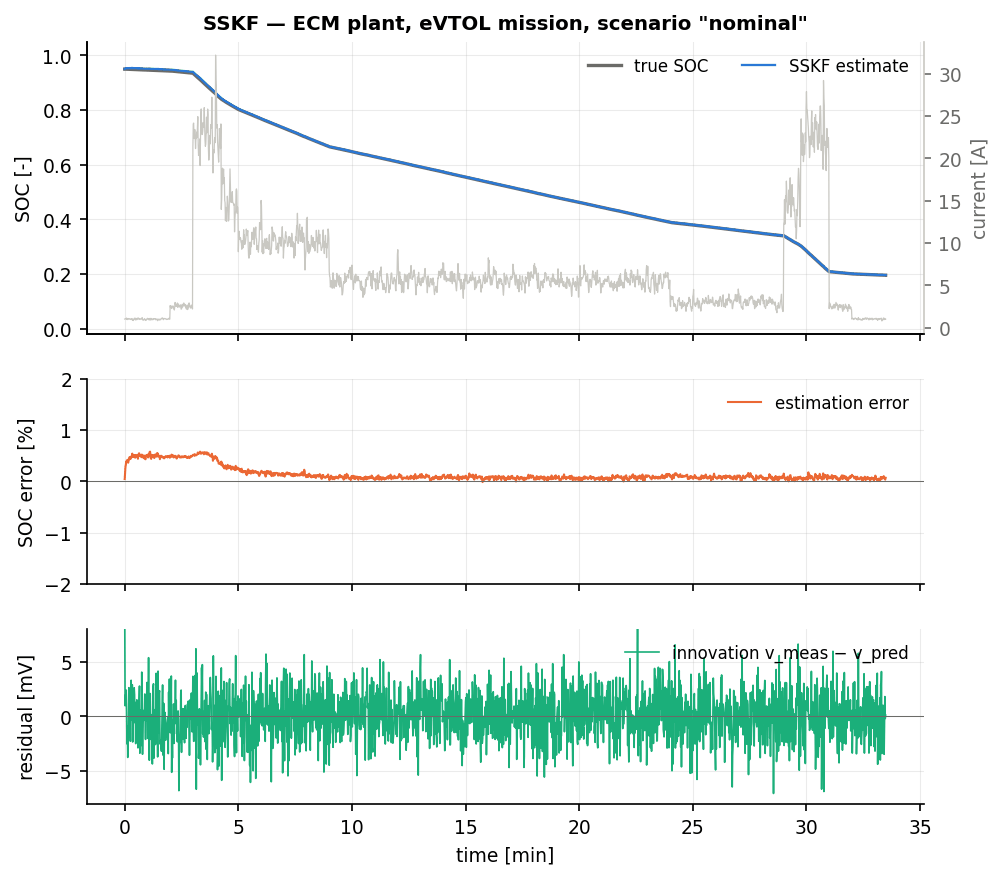
\includegraphics[width=\textwidth]{figures/cell_SSKF_nominal.png}
\caption{SSKF on the nominal eVTOL mission: true and estimated SOC (top), estimation error with the $\pm 2\sigma$ band when available (middle), voltage residual (bottom).}
\end{figure}
\begin{figure}[H]\centering
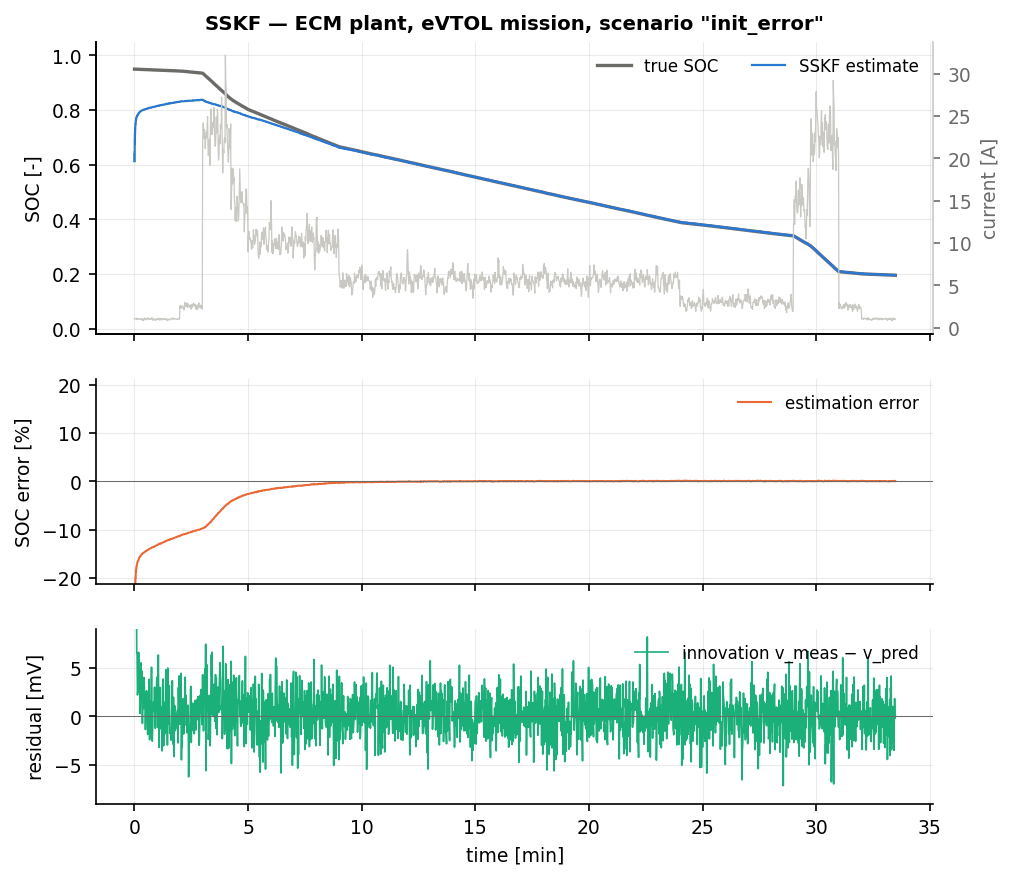
\includegraphics[width=\textwidth]{figures/cell_SSKF_init_error.png}
\caption{SSKF with a 35\,\% initial SOC error.}
\end{figure}

All numbers are over three seeds.  The SSKF reaches $\mathrm{rmse}_{ss}=0.0008$ on
\texttt{nominal} on every seed --- the lowest voltage-residual RMS of the whole observer family
and within a factor of two of the EKF's $0.0005$.  That is the expected result: with the correct
model and the correct noise description, the constant gain is as good as the recursive one in
steady state.  The cost is the transient.  On \texttt{init\_error} the SSKF needs $334$\,s
against the EKF's $0$\,s, because its gain is the stationary one from the first sample; the final
accuracy is then identical ($0.0007$).  This single comparison is the clearest statement of what
the covariance recursion actually buys: nothing in steady state, everything in the transient.

The exact solution of \eqref{eq:lue-dare} matters here more than anywhere else in the family,
because the SSKF \emph{is} that solution.  Iterating the recursion converges linearly at rate
$\rho((\mI-\mK\mC)\mA)^2 \approx 0.9994$ per sweep, so truncating it at a few thousand sweeps does
not give a slightly detuned gain --- it gives the finite-horizon gain of a filter that has only
run for a few thousand samples, and for this plant that gain has the wrong \emph{sign} on the SOC
channel ($L_z=-0.61$ against the converged $+0.066$).  The doubling algorithm removes the question
entirely at $60$--$80$ iterations.

Across the fault scenarios the SSKF tracks the pole-placed observer closely --- to three digits
on most of them, because the certification of \Cref{sec:lue-schedule} rejects the placement on
those scenarios and both registrations then run the same LQE gain (\Cref{ch:luenberger}).  Where
the placement \emph{is} admitted the SSKF is better: \texttt{cold} $0.0031$ against the
Luenberger's $0.0040$, because the LQE design automatically re-weights when the RC time constants
stretch, whereas a fixed pole set asks for the same bandwidth at $-10^\circ$C as at
$25^\circ$C.  \texttt{current\_bias} ($0.0085$), \texttt{aged\_cell} ($0.0218$) and
\texttt{param\_mismatch} ($0.0149$) are all limited by \eqref{eq:lue-ssbias}: the residual bias
is a property of the model error and the OCV slope, not of the gain.  On \texttt{combined} the
SSKF ends at $0.0203$ ($0.0202$--$0.0205$ across seeds) against the EKF's $0.1244$ and no
convergence --- again, a fixed sensible gain degrades far better than a mis-specified optimal one
--- and on the single-particle plant it is at $0.0061$ on \texttt{nominal} and $0.0335$ on
\texttt{cold} against the EKF's $0.0373$ and $0.0735$.

\section{Summary}
Take the SSKF when $\mQ$ and $\mR$ are defensible and the start-up transient is not critical: it
gives EKF-quality steady-state accuracy at a third of the run-time cost and with no covariance
to go indefinite.  Add an explicit process-noise allowance on any integrating channel, because
the model's noise floor there is usually a numerical guard rather than a physical statement.
Avoid it when the measurement noise is strongly non-stationary, when a fast recovery from a bad
initial condition matters, or when a calibrated uncertainty output is required.
